\immediate\write18{makeindex -s nomencl.ist -o Management.nls Management.nlo}

%Layout packages
\documentclass[12pt]{article}
\usepackage[english]{babel}
\usepackage[utf8x]{inputenc}
\usepackage[letterpaper, margin=1.5in,margin=1.2in]{geometry}
\usepackage[colorinlistoftodos]{todonotes}

%Math
\usepackage{amsmath}

%Drawing
\usepackage{graphicx}
\usepackage{epstopdf}
\epstopdfsetup{outdir=./}
\usepackage{tikz}
\usetikzlibrary{shadows,arrows}
% Define the layers to draw the diagram
\pgfdeclarelayer{background}
\pgfdeclarelayer{foreground}
\pgfsetlayers{background,main,foreground}
 
% Define block styles  
\tikzstyle{texture}=[draw, fill=blue!20, text width=6.0em, text centered,
  minimum height=1.5em,drop shadow]
\tikzstyle{diagElt} = [texture, text width=8em, minimum width=10em,
  minimum height=3em, rounded corners, drop shadow]
\tikzstyle{texto} = [above, text width=6em, text centered]
\tikzstyle{linepart} = [draw, thick, color=black!50, -latex', dashed]
\tikzstyle{line} = [draw, thick, color=black!50, -latex']
\tikzstyle{ur}=[draw, text centered, minimum height=0.01em]
 
% Define distances for bordering
\newcommand{\blockdist}{1.3}
\newcommand{\edgedist}{1.5}

\newcommand{\diagElt}[3]{node (p#1) [diagElt]
  {#2\\{\scriptsize\textit{#3}}}}

% Draw background
\newcommand{\background}[5]{%
  \begin{pgfonlayer}{background}
    % Left-top corner of the background rectangle
    \path (#1.west |- #2.north)+(-1,0.6) node (a1) {};
    % Right-bottom corner of the background rectanle
    \path (#3.east |- #4.south)+(+0.6,-0.3) node (a2) {};
    % Draw the background
    \path[fill=yellow!20,rounded corners, draw=black!50, dashed]
      (a1) rectangle (a2);
    \path (a1.east |- a1.south)+(1,-0.35) node (u1)[texto]
      {\scriptsize\textit{#5}};
  \end{pgfonlayer}}

\newcommand{\interOutput}[3]{%
  \path [linepart] (#1.east) -- node [above]
    {\scriptsize interOutput #2} (#3);}

\newcommand{\illu}[3]{%
	\begin{figure}[ht!]
			  \centering
			  \includegraphics[scale=#3]{Graphics/#1}
			  \caption{#2}
			  \smallskip
	\end{figure}}

\newcommand*\emptyPage{\newpage\null\thispagestyle{empty}\newpage}

\usepackage[refpage]{nomencl}
\makenomenclature

\begin{document}

\begin{titlepage}
\newgeometry{top=2cm,bottom=2cm}

\newcommand{\HRule}{\rule{\linewidth}{0.5mm}} % Defines a new command for the horizontal lines, change thickness here

\center % Center everything on the page
 
%----------------------------------------------------------------------------------------
%   HEADING SECTIONS
%----------------------------------------------------------------------------------------


\includegraphics[scale=0.6]{Graphics/logo.png}\\[1.5cm]

\textsc{\Large Projet Electif (technique)}\\[0.5cm] % Major heading such as course name
\textsc{\large Projet technique}\\[0.5cm] % Minor heading such as course title

{\normalsize \today}\\[1.5cm]

%----------------------------------------------------------------------------------------
%   TITLE SECTION
%----------------------------------------------------------------------------------------

\HRule \\[0.4cm]
{ \Large \bfseries Evolution de véhicules autonomes dans un environnement urbain intelligent}\\[0.4cm] % Title of your document
\HRule \\[2.5cm]


%----------------------------------------------------------------------------------------
%   LOGO SECTION
%----------------------------------------------------------------------------------------

 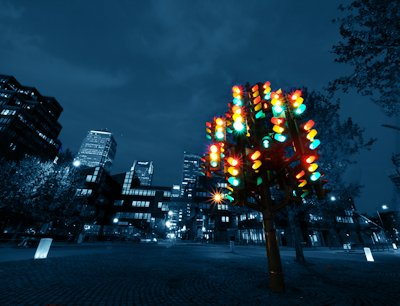
\includegraphics[scale=0.45]{Graphics/illustration.jpg}\\[2.5cm]

%----------------------------------------------------------------------------------------
%   AUTHOR SECTION
%----------------------------------------------------------------------------------------
{\normalsize Auteurs:}\\
\small
\textsc{Biton} Guillaume (guillaume.biton@ipsa.fr)\\
\textsc{Guichard} Marc-Antoine \small(marc-antoine.guichard@ipsa.fr)\\
\textsc{Lhermite} Camille \small(camille.lhermite@ipsa.fr)\\
\textsc{Monnot} Maxime \small(marc-antoine.guichard@ipsa.fr)\\[1cm]

 
%----------------------------------------------------------------------------------------

\vfill % Fill the rest of the page with whitespace

\restoregeometry

\end{titlepage}

\newpage
\tableofcontents
\newpage

\section{Introduction}

	
\newpage
\section{Subdivision of the project}

	

	\begin{center}
	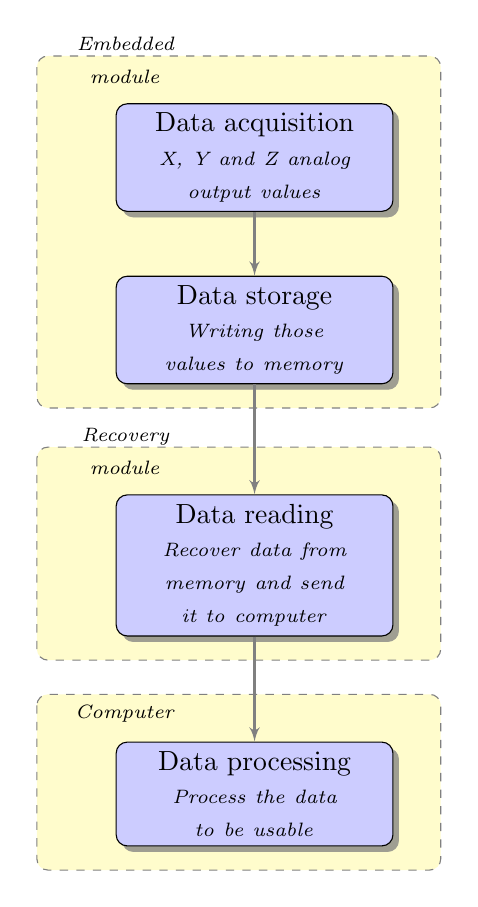
\begin{tikzpicture}[transform shape]
 
  % Draw diagram elements
  \path \diagElt {1}{Data acquisition}{X, Y and Z analog output values};
  \path (p1.south)+(0.0,-1.5) \diagElt{2}{Data storage}{Writing those values to memory};
  \path (p2.south)+(0.0,-2.3)  \diagElt{3}{Data reading}{Recover data from memory and send it to computer};
  \path (p3.south)+(0.0,-2.0) \diagElt{4}{Data processing}{Process the data to be usable};

 
  % Draw arrows between elements
  \path [line] (p1.south) -- node [above] {} (p2);
  \path [line] (p2.south) -- node [above] {} (p3);
  \path [line] (p3.south) -- node [above] {} (p4);
   
  \background{p1}{p1}{p2}{p2}{Embedded module}
  \background{p3}{p3}{p3}{p3}{Recovery module}
  \background{p4}{p4}{p4}{p4}{Computer}
 \end{tikzpicture}

	\end{center}
	
	\nomenclature{SCL}{Serial Clock} \cite{EEPROM}

	\illu{Schematic.png}{Basic input/output schematic}{0.45}

	

\newpage
\section{Conclusion}
	


\newpage
\section{Nomenclature}
	\printnomenclature

\newpage
\section{Bibliography}

	\begin{thebibliography}{9}
	\bibitem{sanchez} 
	Julio Sanchez and Maria P. Canton.
	\textit{Microcontroller Programming: The Microchip PIC}. 
	CRC Press, 2006.
	\end{thebibliography}

\newpage
\section{Appendix}

	\subsection{The GitHub Repository}

		On the GitHub repository of this project (https://github.com/GBhack/UofAmechatronics.git) you will find:
		\begin{itemize}
			\item The Eagle schematics.
			\item The assembly and Matlab codes.
			\item The schematic and code for Arduino testing.
			\item This very document and other team's documentation (which you should probably have a look).
		\end{itemize}

\end{document}